%%
%% HSM: June 2019
%%

\documentclass[English]{article}

%% \usepackage[latin9]{inputenc}
%% \usepackage{babel}
%%
%% other packages
\usepackage[all,cmtip]{xy}
\usepackage{url}
\usepackage{verbatim}
\usepackage{xspace}
\usepackage{amsmath}
\usepackage{amsthm}
\usepackage{thmtools}
\usepackage{amssymb}
\usepackage{color}
\usepackage{float}
\usepackage{graphicx}
\usepackage{mathtools}
\usepackage[square,sort&compress,numbers]{natbib}
\usepackage[top=1in, bottom=1in, left=1in, right=1in]{geometry}
\usepackage[colorinlistoftodos]{todonotes}
\usepackage{hyperref}
\newcommand{\TODO}[1]{\todo[inline,color=red!10,size=\small]{#1}}
\renewcommand\thmcontinues[1]{Continued}
%%
%% ------------------------------------------------------------
\graphicspath{{./}{./Figures/}}
%% ------------------------------------------------------------
%%
\newtheorem{theorem}{Theorem}[section]
\newtheorem{corollary}[theorem]{Corollary}
\newtheorem{lemma}[theorem]{Lemma}
\newtheorem{proposition}[theorem]{Proposition}
%%\theoremstyle{definition}
\newtheorem{definition}[theorem]{Definition}
\theoremstyle{remark}
\newtheorem{remark}[theorem]{Remark}
\newtheorem{example}[theorem]{Example}
%%
\numberwithin{equation}{section}
%%
%% Layout:
\parindent0pt
\parskip6pt
%%
\renewcommand\labelitemi{\rule[0.12em]{0.4em}{0.4em}}
\renewcommand\labelitemii{\normalfont\bfseries \rule[0.15em]{0.3em}{0.3em}}

\def\EpiHiper{EpiHiper\xspace}
\def\EpiHiperVersion{1.0\xspace}
\def\rh#1{\hfill#1\hfill}
\def\thed#1{\textbf{#1}}
\def\hsp{\phantom{$\int\limits_a^b$}}
\def\SciDuct{SciDuct\xspace}

%%
%% Macros:

% Figure size.
\newcommand{\figsize}{0.27}
\newcommand{\expect}{\mathbb{E}}
\newcommand\numberthis{\addtocounter{equation}{1}\tag{\theequation}}
\def\th{\ensuremath{{}^\protect\text{\scriptsize th}}\xspace}

%% ----------------------------------------------------------------------
\begin{document}
%% ----------------------------------------------------------------------
\begin{titlepage}
\raggedleft\raggedbottom
\rule{1pt}{\textheight} % Vertical line
\hspace{0.05\textwidth} % Whitespace between the vertical line and title page text
%%
\parbox[b]{0.75\textwidth}{ % Paragraph box for holding the title page text, adjust the width to move the title page left or right on the page
  {\huge\bfseries NFA Threaded Router:\\[1ex]
    Design, Documentation, \\[1ex] and Scaling Studies}\\[9\baselineskip]
%%
{{\Large\textsc{Author(s):}\\[1ex]
%%
\phantom{\quad}Ryan Jung\\[1ex]
%%
\phantom{\quad}Henning S. Mortveit\\[1ex]
%%
}}\\[4\baselineskip]
%%
{{\Large\textsc{NSSAC Technical Report: No. 2019-TBD}}}\\[2\baselineskip]
%%
{{\Large\textsc{Status: \emph{Approved for NSSAC Internal Release}}}}\\[2\baselineskip]
%%
{{\Large\textsc{Contact:}\\[1ex]\phantom{\quad}Henning S. Mortveit (Henning.Mortveit@virginia.edu)}}\\[2\baselineskip]
%%
{{\Large\textsc{GitHub URL:}\\[1ex]\phantom{\quad}https://github.com/NSSAC/RE\_Router}}\\[7\baselineskip]
%%
\vspace*{\fill}
\vfill
%%
Network Systems Science and Advanced Computing\\
Biocomplexity Institute and Initiative\\
University of Virginia
}
\end{titlepage}
%% ----------------------------------------------------------------------


%%
\title{NFA Threaded Router: \\Design, Documentation, and Scaling Studies}
%%
\author{
Ryan Jung${}^a$ and
%%
Henning S. Mortveit${}^{a,b,\dag}$\footnote{$^\dag$
  Corresponding author: Henning S. Mortveit;\hfil\break
  email: henning.mortveit@virginia.edu;\hfil\break
  github URL: https://github.com/NSSAC/RE\_Router\hfil\break
  NSSAC Technical Report: No. TR 2019--TBD
}\\
%%
\\[1ex]\\
${}^a$Network Systems Science and Advanced Computing;\\
%%
${}^b$Department of Engineering Science and Environment;\\
%%
%%${}^c$Department of Computer Science;\\
%%
%%
University of Virginia
}
\maketitle


%%\keywords{Keywords: To add}
%%
\begin{abstract}
This technical report covers the threaded implementation of the regular
expression (or NFA) constrained router of Jakob et al.

Previously built router using regular expression, was modified to be able to run parallel instances, so that multiple requests could be handled at once.

\end{abstract}
%%

%% ----------------------------------------------------------------------
\section*{Introduction}
\label{sec:introduction}

The algorithm used in this software involved taking an existing NFA and a graph to produce an auxiliary graph. Using this, a Dijkstra's algorthm is used to traverse the graph, but only with the edges of the vertexes have the same edge label that follow with the NFA. This allows for not only traversal with only a specific set of nodes, but allows also for a number of patterns that the program can map out.~\cite{Jacob Constrained Routing.}.

\noindent\fbox{%
    \parbox{\textwidth}{%
        \textsc{Algorithm RE-Constrained-Short-Paths}
        \begin{itemize}
            \item\textit{Input:} A Regular expression \textit{R}, a directed weighted graph \textit{G}, a  source \textit{s}, and a destination \textit{d}
            \item \begin{enumerate}
                \item Construct an NFA
                \item Construct the NFA \textit{M(G)} of \textit{G}
                \item Construct \textit{M(G) X M(R)}. The length of the edges in the product graph is chosen to be equal to the edges in the corresponding graph \textit{G}
                \item Starting from state \textit{(s\textsubscript{0}, s)}, find a shortest path to the vertices \textit{(f, d)}, where \textit{$f \in $F}. Denote these paths by \textit{p\textsubscript{i}}, \textit{$l \leq i \leq $w}. Also denote the cost of \textit{p\textsubscript{i}} by \textit{w(p\textsubscript{i})}.
                \item \textit{C\textsuperscript{*} :=} min\textsubscript{pi}, \textit{w(p\textsubscript{i})}; \textit{p\textsuperscript{*}: w(p\textsuperscript{*}) = C\textsuperscript{*}}.
                (If \textit{p\textsubscript{*} is not uniquely determined, we choose an arbitrary one.}
            \end{enumerate}
            \item \textit{Output:} The path \textit{p\textsuperscript{*}} in \textit{G} from\textit{s} to \textit{d} of minimum length subject to the constraint that of \textit{$l(p) \in $L(R)}
        \end{itemize}
        
    }%
}
\textbf{Report organization.} Section~\ref{sec:design} gives the
software design of the solution Section~\ref{sec:scalingstudies} presents the methodology of the testing and Section~\ref{sec:results} presents the data and possible explanations
Section~\ref{sec:documentation} providing complete user instructions
as well as deploy constructions.



%% ----------------------------------------------------------------------
\section{Design}
\label{sec:design}
The basis of the design takes from the original implementation. Quite simply, the focus is on the critical portion of the code base where:
\begin{itemize}
    \item The NFA is created
    \item The trip requests are processed
    \item The program outputs all the processed request to a text file
\end{itemize}
Taking this, these implementations are stored in a callable method that can be stored in a thread. An additional method needed to be built that takes in the multiple thread requests and splits them up among however many threads the user decides to run. Alongside these changes, many legacy features were removed to help make the program more lightweight and simpler to understand. An option to allocate a certain number of cores was also added for testing purposes.
The idea behind these changes is by allowing for threading and paralleling operations, the program can handle more requests more quickly and efficiently, making full use of a machine's capabilities. 
\begin{figure}[H]
    \centering
    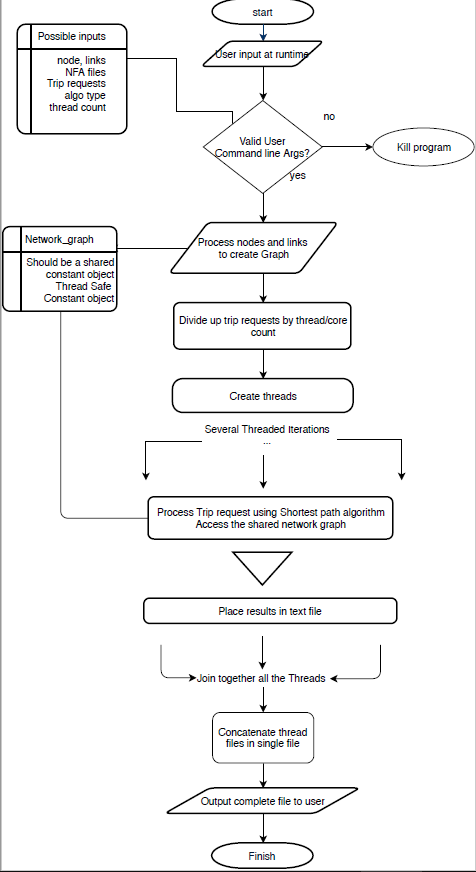
\includegraphics[scale = 0.5]{design.png}
    \caption{Design diagram}
    \label{fig:design1}
\end{figure}

Once these ideas were firmly set out, the critical sections of the code are as follows.

\begin{figure}
    \centering
    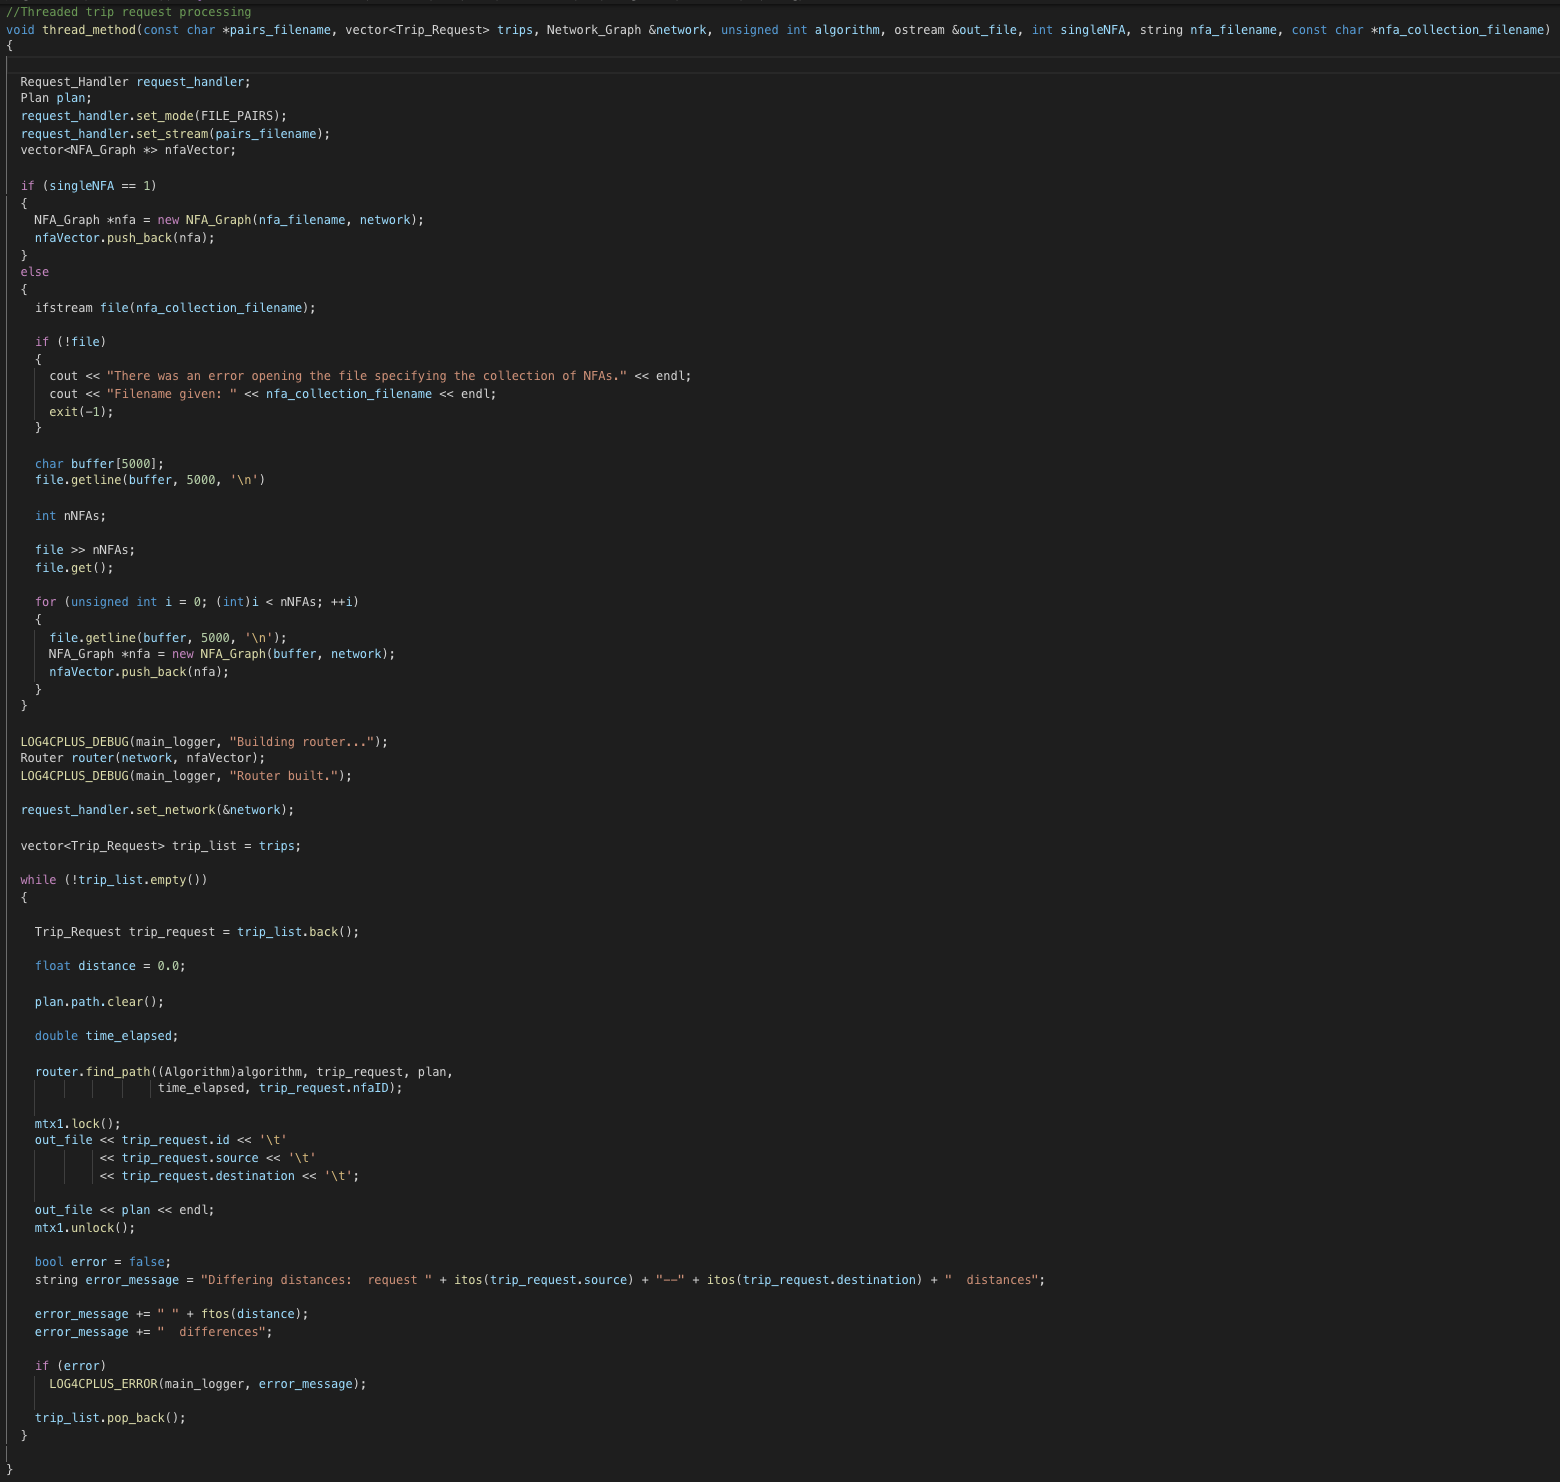
\includegraphics[scale = 0.7]{Code.png}
    \caption{Design diagram}
    \label{fig:code1}
\end{figure}
Compared to the original codebase, it is quite similar, with much of the components being adpated from the original. Major differences include the addition of locks around file output to ensure thread safety.

A custom "Thread Request" method was also created in to work in conjunction with the Thread method. The function of this is to split up a single request across an appropriate number of threads (can be user generated or defaulted to the number of cores existing on the machine) so that the work can be split up among them.

\begin{figure}[!tbp]
  \centering
  \begin{minipage}[b]{0.4\textwidth}
    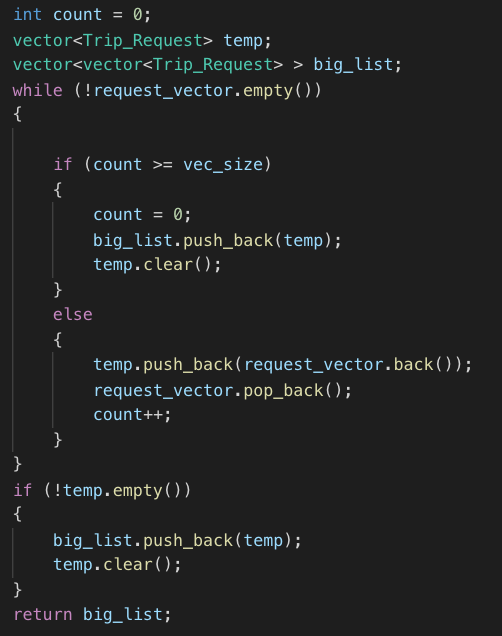
\includegraphics[width=\textwidth]{code1.png}
    \caption{Thread Request.}
  \end{minipage}
  \hfill
  \begin{minipage}[b]{0.4\textwidth}
    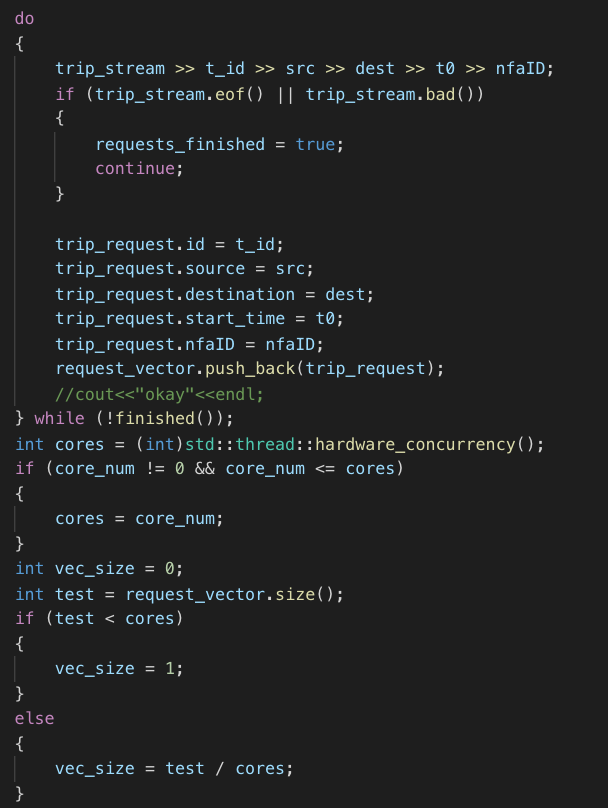
\includegraphics[width=\textwidth]{code2.png}
    \caption{Thread Request cont.}
  \end{minipage}
\end{figure}


%% ----------------------------------------------------------------------
\section{Scaling Studies}
\label{sec:scalingstudies}

Outline of work:
\begin{itemize}
\item Construct e.g. a Python tool that takes as argument the node
  file of a network, and an integer $N$, and that produces a complete
  trip request file containing $N$ random trips. They will all have
  travel mode $0$ which corresponds to automobile. It will likely be
  useful to have trip request files with 1,000, 10,000, and 100,000, requests. For testing, use the smaller request files;
  for the serious scaling studies, use the larger one.
\item Create a timing framework that can time and report the execution
  of the router. It may be helpful to separately time initialization
  code such as construction of networks.
\item Create a timing diagram giving time needed for computation as a
  function of the number of requested compute threads. Conclusions?
  Linear scaling? If not, why not? What happens if you request more
  threads than there are available cores? For each timing run, there
  may be fluctuations due to other computations running on your
  computer/Rivanna. It will likely be useful to at least conduct two
  runs per setting.
\item If time permits, conduct a scaling study on Rivanna using
  multiple nodes.

\end{itemize}

\section{Results}
\label{sec:results}
\begin{figure}[H]
    \centering
    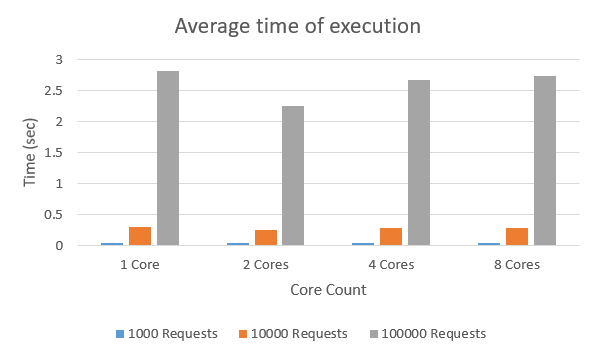
\includegraphics{data.png}
    \caption{Design diagram}
    \label{fig:design1}
\end{figure}

Interestingly, the results show that across the board utilizing only 2 cores would produce the best results. All these tests were performed on a local machine and the only explanation that could be thought of is that the OS is utilizing the other cores for other overhead operation which could cause a slowdown. Further testing on Rivanna with dedicated nodes and cores performing the tests seems like it would be necessary. This was not the expected result where it was initially hypothesized that the relationship between average time and core count would be logarithmic. Still using multiple cores is almost always faster than using one core (save for the test of 1000 trip requests). 

%% ----------------------------------------------------------------------
\bibliographystyle{amsplain}
\bibliography{references}
\begin{thebibliography}{9}
\bibitem{Jacob Constrained Routing.}
Chris Barret, Rico Jacob, and Madhav Marathe
\textit{Formal Language Constrained Path Problems}
Society for Industrial and Applied Mathematics, 2000
\end{thebibliography}
%% ----------------------------------------------------------------------

\cleardoublepage
\appendix

%% ----------------------------------------------------------------------
\section{RE\_Router User Documentation}
\label{sec:documentation}


\begin{verbatim}
./new_main -g <graph> -c <coords> -N <NFAFILE> -s <cores> -t <time> -f <pairs>

  -c <coords>: coordinates (vertex) file
  
  -g <graph>: pairs from file

  -N <NFAFile>:graph (edge) file

  -s <cores>: specifiying how many cores (and consequently threads) are used
  
  -t <time>: time of departure
  
 plans.txt: output file returning request path traversal
 
./trip_maker.py: prompts user for a number and creates that many trip requests

./super_script.sh:runs program with newly created pairs file from trip_maker.py with 4 cores

./testing_frame: prompts user for number of requests and number of cores. 
   Runs 100 trials and returns the average time and all trial times to a .csv file

./data_collect.py: runs 3 tests of 1000, 10,000, and 100,000 requests. Returns 3
   .csv files with results

  
\end{verbatim}


%% ----------------------------------------------------------------------


\subsection{Input Files}
\label{sec:inputfiles}

The router uses the following input files:
\begin{itemize}
\item Network node file: The text file with specifications of node id and travel options
\item Network link file: The text file that puts together the nodes
\item Trip Request file: The text file that puts out specific travel routes
\end{itemize}




\end{document}
